\documentclass[
    % draft,                             % 草稿模式
    aspectratio=169,                   % 使用 16:9 比例
]{beamer}
\mode<presentation>
\usetheme[
    % navigation=subsections,            % 使用子章节进度显示
    % lang=en,                           % 使用英文
    % cjk=true,                          % 使用CJK而不是ctex
    color=red,                         % 使用红色主题
    % pattern=all,                        % 使用全图案装饰
    % gbt=bibtex,                        % 使用 gbt (使用 bibtex 编译)
]{sjtubeamermin}
\usecolortheme[]{beaver}                 % 使用其他颜色主题
\addbibresource{ref.bib}               % gbt!=bibtex

\begin{document}
    % \institute[School of Electrical Engineering]{数学科学学院}   % 组织
    \institute[Department of Automation]{自动化系}   % 组织
    \logo{
        
\includegraphics{cnlogored.pdf}  % 重定义 logo
    }
    \titlegraphic{                         % 标题图像
        \begin{stampbox}
            
\includegraphics[width=0.3\textwidth]{coffeemaker.jpeg}
        \end{stampbox}
    }
    \title{Assignment 1: Coffeemaker control system}  % 标题
    \subtitle{IoT application system development}         % 副标题
    \author{Pedro Hernández Rubio (021032990002)}                  % 作者
    \date{\today}                          % 日期  
    \maketitle                             % 创建标题页

\part{第一部分 IoT application system development}

% 使用节目录
\AtBeginSection[]{
    \begin{frame}
        % \tableofcontents[currentsection]           % 传统节目录             
        \sectionpage                   % 节页
    \end{frame}
}

% 使用小节目录
% \AtBeginSubsection[]{                  % 在每小节开始
%     \begin{frame}
%         \tableofcontents[currentsection,currentsubsection]             % 传统小节目录             
%         \subsectionpage                % 小节页
%     \end{frame}
% }

\section{第 1 节 The IoT idea}

\subsection{第 1 小节 Context: coffeemakers' health}

    \begin{frame}
        \frametitle{Context: coffeemakers' health}

        \begin{block}{Problem}
            I am addicted to drinking coffee. I should quit as it is not good for health but it is not easy. Anyways, I have already broken (burnt) a couple of coffeemakers: I start boiling the coffeemaker but I forget putting it out in time... 咖啡机坏了! I am quite absent-minded...
        \end{block}

        \begin{block}{Solution}
            I need a real-time communication system for safety, in order to send me an alert as soon as coffee is ready. So that I can quickly put coffeemaker out kitchen fire, avoiding burnt coffee and damages to coffeemaker. Optimally, receiving an alert message to my mobile phone.
        \end{block}

    \end{frame}

\subsection{第 2 小节 Context: general project design}

    \begin{frame}
        \frametitle{General project design}

        \paragraph{Goal} Getting temperature to cloud IoT platform for data processing

        \begin{figure}
            \centering
            \begin{stampbox}
                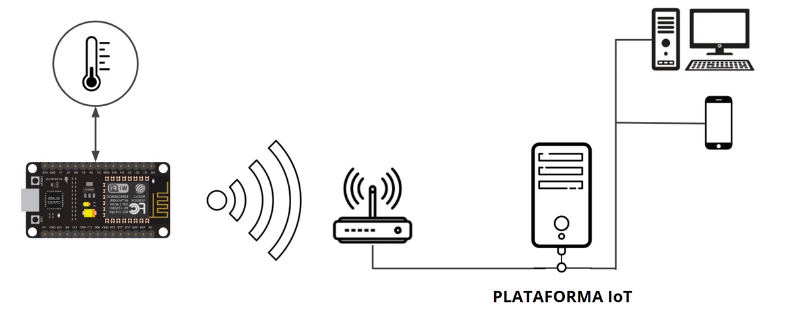
\includegraphics[height=0.5\textheight]{esquema-general.png}
            \end{stampbox}
            \caption{IoT device sends data through WiFi connection}
        \end{figure}

    \end{frame}

\section{第 2 节 Components}

\subsection{第 1 小节 Hardware components}

    \begin{frame}
        \frametitle{Hardware components}

        \paragraph{Goal} Connecting board with sensor temperature 

        \begin{itemize}
            \item \alert{NodeMCU\cite{nodemcu}}: low-cost open source IoT board with ESP8266 SoC
            \item \alert{Temperature sensor DS18B20\cite{ds18b20}}: for non-constrained resources (without memory problems)
            \item \alert{Power supply module MB102}: low-cost 3.3V$\sim$5V supply
            \item \alert{Others:}
            \begin{itemize}
                \item \alert{Breadboard}: for components' wiring and fixing
                \item \alert{Resistor}: 5.1K (4.7K recommended for sensor)
                \item \alert{USB to microUSB adapter}: uploading code to flash memeory in board      
            \end{itemize}
        \end{itemize}

    \end{frame}

\subsection{第 2 小节 Software components}

    \begin{frame}
        \frametitle{Software components}

        \paragraph{Goal} Coding setup for code uploading to the board

        \begin{itemize}
            \item \alert{Linux Mint OS}: Linux OS distribution based in Ubuntu flavour.
            \item \alert{Arduino IDE\cite{arduinoide}}: Version 1.8.16 for Linux OS distributions. NodeMCU is a so popular electronic board that Arduino IDE provides support for it. Same core and external libraries for Arduino programming environment are available.
        \end{itemize}

    \end{frame}

\section{第 3 节 Development}

\subsection{Phase 1: IoT device setup}

    \begin{frame}
        \frametitle{Phase 1: Setup - IoT device}

        \begin{columns}[T,onlytextwidth]
            \column{0.4\textwidth}
              \begin{block}{IoT device setup}
                    Connection between NodeMCU board and sensor DS18B20 through 3 wires: data pin D5 (read temperature), ground and supply.
                \end{block}
                \begin{block}{[optional] power supply}
                    For IoT device autonomy, a power supply MB102 can be attached to the device (Supplying around 3.3V an 5.V for the sensor,  higher power could produce damages)
                \end{block}
            \column{0.5\textwidth}
            \begin{figure}
                \centering
                \begin{stampbox}
                    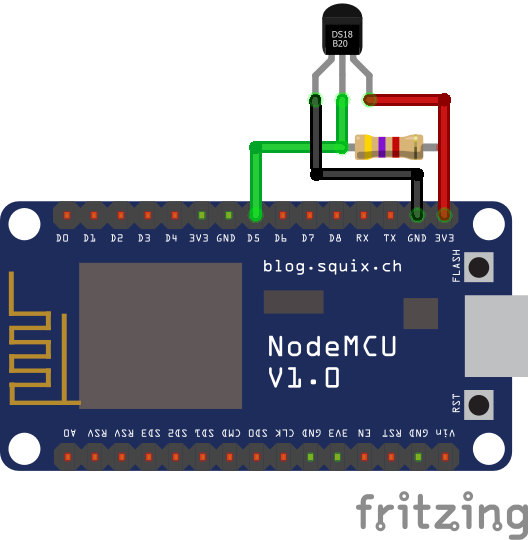
\includegraphics[height=0.6\textheight]{funnel-esp8266-3.png}
                \end{stampbox}
                \caption{NodeMCU and DS18B20}
            \end{figure}        
        \end{columns}

    \end{frame}

\subsection{Phase 1: Arduino IDE config}

    \begin{frame}
        \frametitle{Phase 1: Setup - Arduino IDE config}
        
        \paragraph{Board manager} Install \alert{esp8266} support (from ESP8266 Community)

        \paragraph{Select board} Tools -> NodeMCU 1.0 (ESP 12-E Module)

        \paragraph{Arduino IDE} Other board settings: 

        \begin{itemize}
            \item \alert{Upload rate}: 115200 (not fast but reliable)
            \item \alert{Flashing size}: 4MB (2MB for filesystem)
            \item \alert{Port}: /dev/ttyUSB0 (Linux USB)
        \end{itemize}

        \begin{block}{Serial communication}
            Through wire USB (laptop) to microUSB (board) -> allowing code uploading to Flash memory (after compilation) and serial monitor communication
        \end{block}
    \end{frame}

\subsection{Phase 1: Software libraries}

    \begin{frame}[fragile]          % 注意添加 fragile 标记
        \frametitle{Phase 1: Setup - Software libraries}
        % 代码块参数:语言,标题
        % 请减少代码初始的缩进
        \begin{codeblock}[language=c]{C代码}
#include <OneWire.h> // For one wire communication with sensor DS18B20
#include <DallasTemperature.h> // For sensor DS18B20 (propietary enterprise)
#include <ESP8266WiFi.h> // For WiFi connection management
#include <ESP8266HTTPClient.h> // API for easy HTTP requests
#include <ThingSpeak.h> // Cloud IoT platform
        \end{codeblock}
    \end{frame}

\subsection{Phase 2: IoT platform (ThingSpeak)}

    \begin{frame}
        \frametitle{Phase 2: IoT platform (ThingSpeak) - System design}

        \begin{columns}[T,onlytextwidth]
            \column{0.4\textwidth}
              \begin{block}{ThingSpeak\cite{thingspeakchannel} features}
                Main advantages of this IoT platform:
                \begin{itemize}
                    \item \alert{Database}: storing data
                    \item \alert{Graphing}: advanced statistics
                    \item \alert{Dashboard}: real-time IoT information
                \end{itemize}
              \end{block}
            \column{0.5\textwidth}
            \begin{figure}
                \centering
                \begin{stampbox}
                    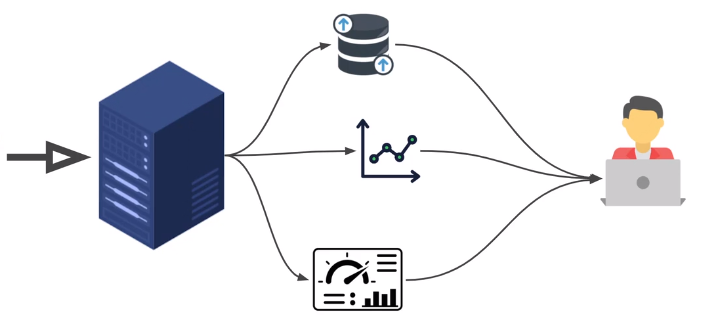
\includegraphics[height=0.3\textheight]{thingspeak-schema.png}
                \end{stampbox}
                \caption{IoT platform}
            \end{figure}       
        \end{columns}

    \end{frame}

\subsection{Phase 2: IoT platform (ThingSpeak) - Data channel (public)}

    \begin{frame}
        \frametitle{Phase 2: IoT platform (ThingSpeak) - Data channel}

        \paragraph{Install} ThingSpeak library (by MathWorks) for easy coding

        \begin{columns}[T,onlytextwidth]
            \column{0.4\textwidth}
              \begin{block}{Coffemaker channel}
                \begin{itemize}
                    \item \alert{Channel ID:}: 1554737
                    \item \alert{Data field}: temperature
                    \item \alert{Access}: public\cite{thingspeakchannel}
                \end{itemize}
              \end{block}
            \column{0.5\textwidth}
            \begin{figure}
                \centering
                \begin{stampbox}
                    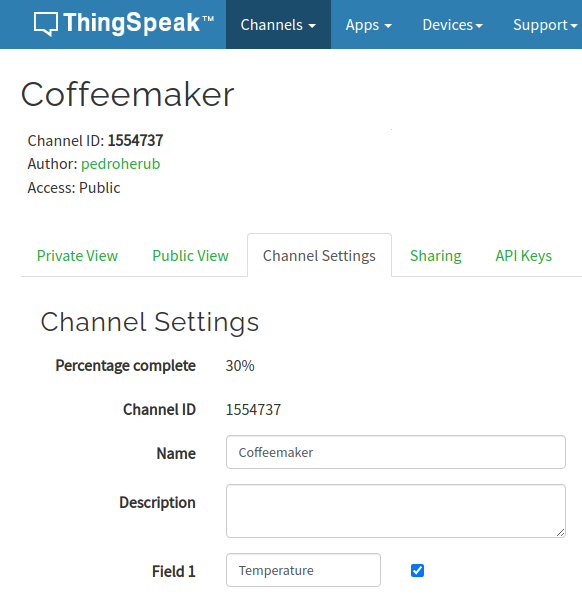
\includegraphics[height=0.5\textheight]{thingspeak-channel.png}
                \end{stampbox}
                \caption{Public channel info}
            \end{figure}        
        \end{columns}

    \end{frame}

\subsection{Phase 2: IoT platform (ThingSpeak) - Sending sensor data}

    \begin{frame}
        \frametitle{Phase 2: IoT platform (ThingSpeak) - Sending sensor data}

        \paragraph{ThingSpeak dashboard} Coffemaker spent when coffee was boiled ($\sim$90 degrees)

        \begin{figure}
            \centering
            \begin{stampbox}
                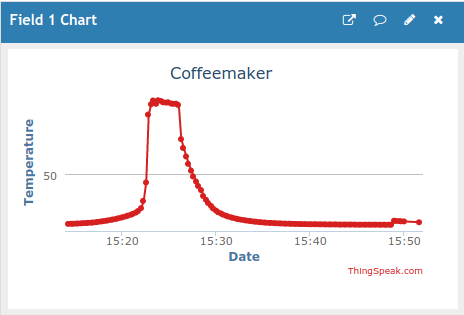
\includegraphics[height=0.5\textheight]{thingspeak-coffeemaker.png}
            \end{stampbox}
            \caption{Coffeemaker lifycycle}
        \end{figure}
        
    \end{frame}

\subsection{Phase 3: Node-RED manager - Deployment}

    \begin{frame}
        \frametitle{Phase 3: Node-RED manager - Deployment}

        \begin{block}{Node-RED as IoT network brain}
            Intercommunicating and orchestrating different IoT devices and cloud solutions (solving the lack of standarization among IoT vendors)
        \end{block}

        \paragraph{Deployment} Posible solutions:

        \begin{block}{Options}
            \begin{itemize}
                \item \alert{Local network deployment}: Raspberry Pi (common solution)
                \item \alert{Cloud hosted node}: FRED\cite{servicesFred} (chosen solution)
            \end{itemize}
        \end{block}

        \begin{block}{FRED}
            Frontend for Node-RED manages instances of Node-RED for multiple users in the cloud
        \end{block}

    \end{frame}


\subsection{Phase 3: Node-RED manager - Graphical flow}

    \begin{frame}
        \frametitle{Phase 3: Node-RED manager - Graphical flow (I)}

        \paragraph{Tool} Web code editor (mostly graphical for simple projects)

        \begin{figure}
            \centering
            \begin{stampbox}
                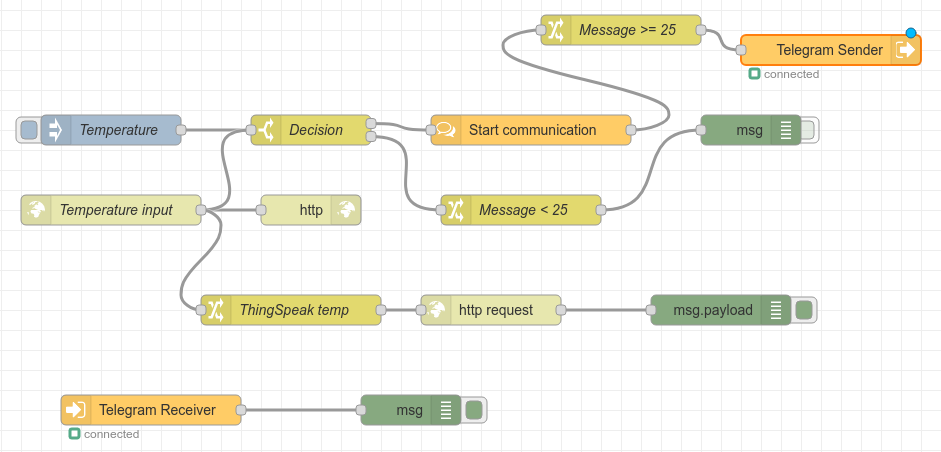
\includegraphics[height=0.5\textheight]{nodered-flow.png}
            \end{stampbox}
            \caption{Flow management}
        \end{figure}
        
    \end{frame}

\subsection{Phase 3: Node-RED manager - Graphical flow}

    \begin{frame}
        \frametitle{Phase 3: Node-RED manager - Graphical flow (II)}

        \paragraph{API endpoint} External requests (from IoT devices) initialize the whole process by sending sensor data to this input API receiver. Example: \url{https://pedroherub.fred.sensetecnic.com/api/public/temperature?temp=25}

        \begin{block}{Decision process}
            IoT device send temperature data to the Node-RED instance each 16 seconds. Performing decision:
            \begin{itemize}
                \item \alert{Coffee not ready}: Temperature $<=$ 90 degrees (wait)
                \item \alert{Coffe finished!}: Temperature $>$ 90 degrees (alert message)
            \end{itemize}
        \end{block}
        
    \end{frame}

\subsection{Phase 3: Node-RED manager - Serial monitor}

    \begin{frame}
        \frametitle{Phase 3: Node-RED manager - Serial monitor}

        \begin{figure}
            \centering
            \begin{stampbox}
                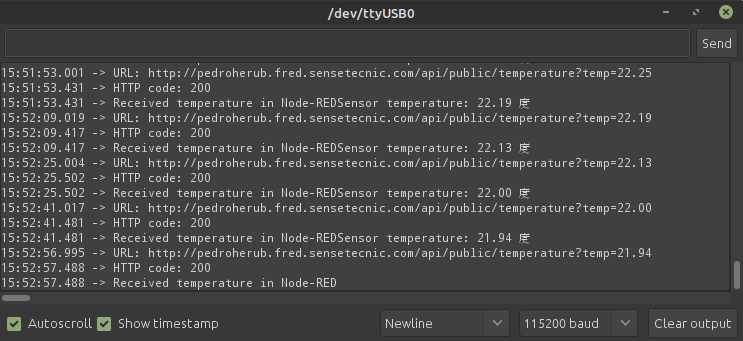
\includegraphics[height=0.5\textheight]{serial-monitor.png}
            \end{stampbox}
            \caption{Data monitor: process info from serial USB}
        \end{figure}

    \end{frame}

\subsection{Phase 4: Telegram bot - Web service configuration}

    \begin{frame}
        \frametitle{Phase 4: Telegram bot - Web service configuration}

        \begin{block}{Node-RED as IoT network brain}
            Intercommunication and orchestrating different IoT devices and cloud solutions
        \end{block}

        \paragraph{Goal} Components classification:

        \begin{block}{Options}
            \begin{itemize}
                \item \alert{Local network deployment}: Raspberry Pi (common solution)
                \item \alert{Cloud hosted node}: Fred
            \end{itemize}
        \end{block}

    \end{frame}

\subsection{Phase 4: Telegram bot - Flow integration}

    \begin{frame}
     \frametitle{Phase 4: Telegram bot - Flow integration}
        \begin{figure}
            \centering
            \begin{stampbox}
                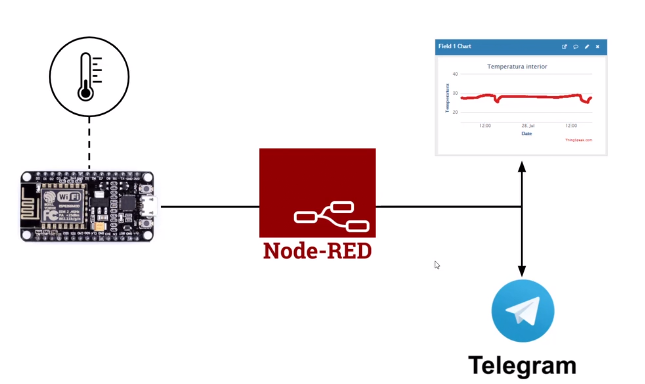
\includegraphics[height=0.5\textheight]{nodered-telegram.png}
            \end{stampbox}
            \caption{Decentralized Access Control Architecture}
        \end{figure}

        \begin{block}{Importing and exporting}
            Access control management information is stored in the blockchain layer.
        \end{block}
    \end{frame}

\subsection{Phase 4: Telegram bot - Sending data to ThingSpeak from Node-RED}

    \begin{frame}
        \frametitle{Phase 4: Telegram bot - Sending data to ThingSpeak from Node-RED}
        \begin{figure}
            \centering
            \begin{stampbox}
                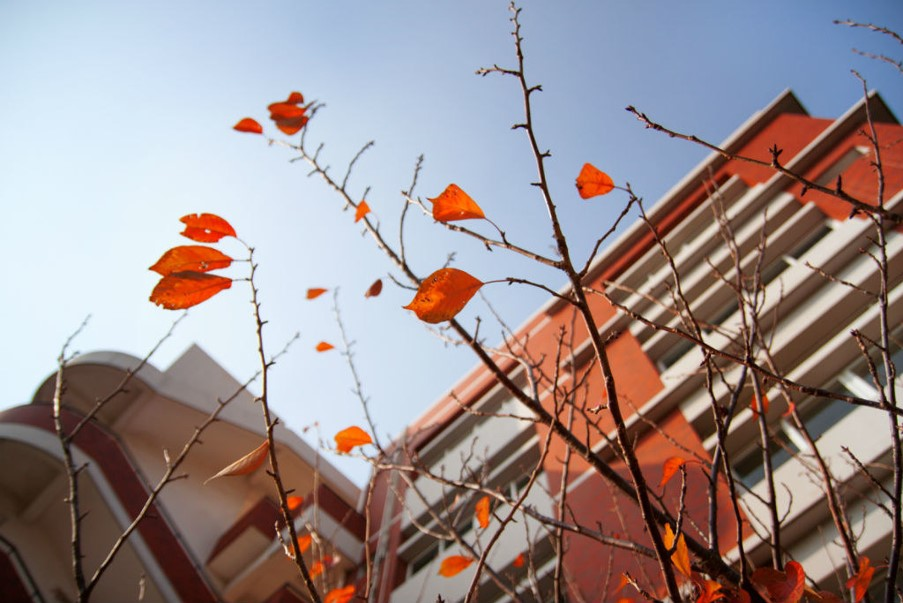
\includegraphics[height=0.3\textheight]{plant.jpg}
            \end{stampbox}
            \caption{图片标题}
        \end{figure}
    \end{frame}

\subsection{Issues: hardware}

    \begin{frame}
        \frametitle{Issues: hardware}

        \begin{block}{Hardware: resistor 4.7K}
            After buying a starter electronic kit, I realized there was no 4.7K resistor included (recommended\cite{resistor} for sensor DS18B20). I was afraid of damaging electronic components
        \end{block}

        \begin{block}{Possible solutions}
            \begin{itemize}
                \item \alert{Parallel resistors}: 2 10K resistors
                \item \alert{Serial resistors}: several resistors adding about 4.7K
            \end{itemize}
        \end{block}

        \begin{block}{Final solution: power supply MB102}
            When connecting a power supply module to the breadboard, energy supply is more accurate ($\sim$5V). Then, an exact resistor value is not so important. A 5.1K resistor is good enough (some tolerance in limits)
        \end{block}

    \end{frame}

\subsection{Issues: software}

    \begin{frame}
        \frametitle{Issues: software}

        \begin{block}{Software: kernel module CH341}
            Initially my Linux OS was not recognizing NodeMCU board through USB wire. Finally I found solution.\cite{ch341} I needed to update a kernel module \alert{ch341.c} in charge or serial USB communication:
            \begin{enumerate}
                \item Downloading kernel module new source
                \item Compiling the kernel module
                \item Upgrading the current loaded kernel module
            \end{enumerate}
        \end{block}

% \begin{codeblock}[language=bash,numbers=none]{Shell命令}
% echo a
% \end{codeblock}

    \end{frame}


    % \begin{frame}
    %     \frametitle{Extra}

    %     \begin{columns}[T,onlytextwidth]
    %         \column{0.4\textwidth}
    %         \metroset{block=fill}
    %           \begin{exampleblock}{UI}
    %             Estilo similar a Google Calendar
    %           \end{exampleblock}
    %           \begin{exampleblock}{Acciones}
    %             \begin{itemize}
    %                 \item Crear nueva
    %                 \item Ver detalle
    %                 \item Actualizar
    %                 \item Eliminar
    %             \end{itemize}
    %           \end{exampleblock}
    %           \begin{exampleblock}{Bonus}
    %             Drag \& resize
    %           \end{exampleblock}
    %         \column{0.5\textwidth}
    %         \begin{center}
    %             \includegraphics[height=.7\textheight]{balsamiq/calls1.png}\hfill
    %         \end{center}
            
    %     \end{columns}
        
    %     \begin{multicols}{2}
    %     \begin{table}
    %         \caption{表格标题}
    %         \pgfplotstabletypeset[
    %             columns/Quick/.style={dec sep align},
    %             columns/Cocktail/.style={dec sep align},
    %             column type=r,
    %             % fixed zerofill,
    %         ]{test.csv}
    %     \end{table}
        
    %     \begin{figure}
    %         % !TeX root = ../main.tex
% Made with PGFPlotsEdt:
% https://logcreative.github.io/PGFPlotsEdt/
\begin{tikzpicture}
    \begin{axis}[
    height=0.45*\the\paperheight,
    xlabel={$n$},
    ylabel={Average Steps},
    ymin={0},
    xmax={9},
    xmin={1},
    legend style={at={(0.5,1.05)},anchor=south},
    legend columns=2,
    grid,
    minor tick num=1]
     \pgfplotstableread {test.csv}{\foo};           % read table
     \addplot+ [only marks,mark options={scale=0.8}] table[y=Quick] {\foo};
     \addplot+ [only marks,mark options={scale=0.8}] table[y=Cocktail] {\foo};
     \pgfplotsset{cycle list shift=-2};                 % start the cycle list from beginning
     \addplot+ [no markers,domain=1:9,] {1.502*x*ln(x)};
     \addplot+ [no markers,domain=1:9,] {0.4453*x*x-0.1365*x-0.473};
     \legend{Quick,Cocktail,}                           % only mark the first two series
    \end{axis}
\end{tikzpicture}
    %         \caption{统计图标题}
    %     \end{figure}
    %     \end{multicols}
    % \end{frame}


% gbt=bibtex
\part{References 参考文献}
    \begin{frame}[allowframebreaks]
        \printbibliography[title=References 参考文献]    % gbt!=bibtex
        % \bibliography{ref.bib}             % gbt=bibtex
    \end{frame}

    \makebottom     % 创建尾页  % 非标准命令

\end{document}